\documentclass[final]{beamer}
\usepackage{beamerposter}
\usepackage{booktabs}
\usepackage{amssymb}
\usepackage{listings}
\usepackage{courier}
\usepackage{float}
\usepackage{graphicx}
\usepackage{caption}
\usepackage{fontawesome}
\usepackage[scale=2]{ccicons}
\usepackage{hyperref}
\usepackage[backend=biber]{biblatex}
\addbibresource{refs.bib}

% lorem ipsum packages
\usepackage[english]{babel}
\usepackage{blindtext}
\usepackage{lipsum}


% styling commands - template from http://www.latextemplates.com/cat/conference-posters
\usetheme{confposter}
% \setbeamercolor{}{}
\usefonttheme{professionalfonts}
\setbeamerfont{block body}{series=\sffamily, size={\fontsize{32}{36}}}
\addtobeamertemplate{block end}{}{\vspace*{4ex}} % White space under blocks
\addtobeamertemplate{block alerted end}{}{\vspace*{4ex}} % White space under highlighted (alert) blocks


% layout
% 4-column layout, separation width = 0.008 of paper width
% onecolwid = (1-((4+1)*sepwid))/4 e.g. (1-((4+1)*0.008))/4 = 0.24
% Set twocolwid to be (2*onecolwid)+sepwid = 0.488
\newlength{\sepwid}
\newlength{\onecolwid}
\newlength{\twocolwid}
\setlength{\sepwid}{0.04\paperwidth} % Separation width (white space) between columns
\setlength{\onecolwid}{0.2\paperwidth} % Width of one column
\setlength{\twocolwid}{0.44\paperwidth} % Width of two columns
\setlength{\topmargin}{-0.5in} % Reduce the top margin size


% document metadata
\title{Visualizing Mobile Phone Sensor Data in an R Environment}
\author{Riccardo Miccini}
\institute{Technical University of Denmark - DTU}
\date{\today}


% begin document - single frame, multi-column layout
\begin{document}
\begin{frame}[t]
\begin{columns}[t]

% column 1 - left
\begin{column}{\onecolwid}
	% objectives
	\begin{alertblock}{Objectives}
		The aim of the project is the application of methods for visualizing mobile phone (Android, iPhone) sensor measurements in an R environment, using the \emph{Google Cloud} as buffer.
		The system has to be able to:
		\begin{itemize}
			\item Collect GPS positioning data from mobile phones and store them remotely.
			\item Read the content of the spreadsheet from an R environment in real-time, and visualize spatial data on a map and other information on plots.
			\item Allow the user to interact with the data - filtering, zooming, scrolling, exporting\dots
		\end{itemize}
	\end{alertblock}

	% intro
	\begin{block}{\faCommenting \, Introduction}
		The project has been carried out under the supervision of profs. John Aasted S{\o}rensen and Ian Bridgwood, as part of a multidisciplinary project.

		The implemented system is composed of three main elements: a series of end users' mobile devices, a remote host, and a \emph{data analyst} station.
		The former are equipped with a custom-made application capable of submitting GPS data to a remote \emph{Google Sheet} document, which acts as a database and is accessible through the cloud.
		The data analyst can then visualize the collected data in real-time, using the provided R scripts and a web browser.

		\bigskip

		\small{\emph{All brands, product names, logos, or other trademarks featured or referred to in this document are the property of their respective holders, and their use does not imply endorsement.}}
	\end{block}

	% reqs
	\begin{block}{\faListUl \, Requirements}
		Here is a summarization of the \emph{Software Requirements Specification}:
		\begin{itemize}
			\item The collected data shall include device ID, coordinates (latitude, longitude), altitude, speed, and timestamp.
			\item The mobile phone app shall submit data at a user-defined time interval.
			\item The R software shall visualize the spatial information using a map and any other data using a chart, in real-time.
			\item All the developed source code should be modular, reusable, and well-documented.
		\end{itemize}
	\end{block}
\end{column}

% column 2 - center
\begin{column}{\twocolwid}
	\begin{columns}[t, totalwidth=\twocolwid]
		% column 2.1 - centerleft
		\begin{column}{\onecolwid}\vspace{-.6in}
			% tools
			\begin{block}{\faWrench \, Tools}
				R is an open-source programming language and software environment for statistical computing, data analysis, and visualization.

				\blindlist{itemize}[4]
				\lipsum[66]
			\end{block}
		\end{column}

		% column 2.2 - centerright
		\begin{column}{\onecolwid}\vspace{-.6in}
			% implementation
			\begin{block}{\faCode \, Implementation}
				\blindtext
				\lipsum[75]
				\lipsum[66]
			\end{block}
		\end{column}
	\end{columns}

	% main figure section
	\begin{figure}
		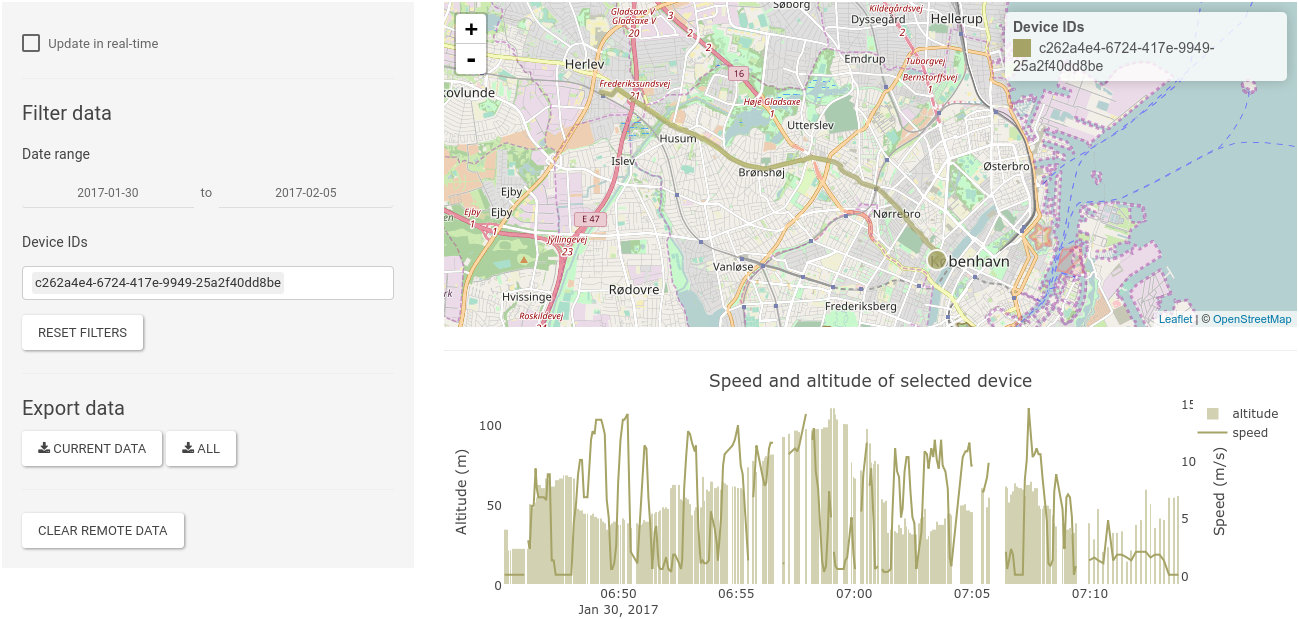
\includegraphics[width=\twocolwid]{ss_ui.png}
		% \caption{Figure caption}
	\end{figure}

	% copyright notice
	\vspace{2cm}

	\begin{center}
		\ccbynd
	\end{center}
\end{column}

% column 3 - right
\begin{column}{\onecolwid}
	% testing
	\begin{block}{\faCheckCircle \, Verification}
		\lipsum[75]
		\lipsum[66]
	\end{block}

	% conclusion
	\begin{block}{\faPieChart \, Results and Conclusion}
		\blindtext
	\end{block}

	% refs
	\begin{block}{\faPaperclip \, References}
		\nocite{*}
		\small{\printbibliography}
	\end{block}

	% contacts
	\begin{alertblock}{ Conctact Information}
		\faUser \, Riccardo Miccini \\
		\faEnvelope \, s137345@student.dtu.dk \\
		\faGithub \, miccio-dk \\
		\faLinkedin \, rimiccini
	\end{alertblock}

\end{column}

\end{columns}
\end{frame}
\end{document}
